\documentclass[11pt,a4paper]{article}
\textheight245mm
\textwidth170mm
\hoffset-21mm
\voffset-15mm
\parindent0pt
\usepackage[utf8]{inputenc}
\usepackage{dsfont}
\usepackage{graphicx}
\usepackage{caption}
\usepackage{fancyhdr}
\usepackage{mathdots}	
\usepackage{amsmath,amsfonts,amssymb}
\usepackage[french]{babel}
\usepackage[maxalphanames=99, maxnames=99, backend=bibtex, style=alphabetic, sorting=ynt]{biblatex}
\addbibresource{cex-denjoy.bib}
\usepackage[hidelinks]{hyperref} 
\hypersetup{
  colorlinks   = true,    % Colours links instead of ugly boxes
  urlcolor     = blue,    % Colour for external hyperlinks
  linkcolor    = black,   % Colour of internal links
  citecolor    = black    % Colour of citations
}
\usepackage{../zephyr}
\pagestyle{fancy}

\usepackage{array,multirow,makecell}
\setcellgapes{4pt}
\makegapedcells
\newcolumntype{R}[1]{>{\raggedleft\arraybackslash }b{#1}}
\newcolumntype{L}[1]{>{\raggedright\arraybackslash }b{#1}}
\newcolumntype{C}[1]{>{\centering\arraybackslash }b{#1}}

\renewcommand{\headrulewidth}{1pt}
\fancyhead[C]{}
\fancyhead[L]{L3 - 2023/2024}
\fancyhead[R]{D.E.R Mathématiques}

\renewcommand{\footrulewidth}{1pt}
\fancyfoot[C]{\thepage} 
\fancyfoot[L]{Sacha Ben-Arous}
\fancyfoot[R]{E.N.S Paris-Saclay}

\title{\textbf{Contre-exemples au théorème de Denjoy }}
\date{}


\begin{document}
\maketitle

\ \ \ \ \ Ce document est consacré à l'étude de certains contre-exemples du théorème de Denjoy. Dans une première partie nous construirons des contre-exemples de régularité optimale, dus à Denjoy, et qui sont développé par Michael Herman dans sa thèse \cite{herman}, en particulier au chapitre X. Nous présenterons ensuite un résultat sur la densité de ces contre-exemples, en suivant toujours les travaux de Herman.
\section{Introduction et outils}

On se propose de montrer le théorème suivant :

\begin{theorem}\textbf{(Denjoy) : }
Pour tout $\alpha \in \mathbb{R} \setminus \mathbb{Q}$, $\forall \epsilon > 0$, il existe un $\mathcal{C}^{2-\epsilon}$-difféomorphisme $f$ du tore tel que $\rho(f)=\alpha$ et $f$ n'est pas conjugué à la rotation $R_\alpha$.
\end{theorem}

~\\
\underline{Rq }: Ici, la  régularité non-entière est définie au sens de Hölder, i.e $f$ est $\mathcal{C}^1$, de dérivée $1-\epsilon$-hölderienne.\\

\ \ \ \ \ Pour construire un contre-exemple, on s'inspire de la preuve du théorème dans le cas $\mathcal{C}^2$ : on sait déjà par Poincaré qu'un tel $f$ est semi-conjugué à $R_\alpha$ par une fonction continue croissante $h$ du tore. La preuve procède par l'absurde, en montrant que si $h$ n'est pas inversible, alors elle est constante sur un intervalle $I$ non trivial du tore. Les itérés $f^n(I)$ sont alors disjoints (on dit que $I$ est un intervalle errant pour la dynamique de $f$), et on conclut en montrant que la somme de leurs tailles diverge. \\ 
L'idée ici est donc construire une fonction $f$ qui admet un intervalle errant mais dont la suite des tailles des itérés est sommable. \\

On se servira de l'invariant de conjuguaison suivant : 

\begin{defin} : Un homéomorphisme du tore $f$ est dit \textit{minimal} si tout ensemble fermé invariant par  $f$ est vide ou égal au tore tout entier. 
\end{defin}

\label{prop:mini}
\begin{proposition} ~ 
\begin{enumerate}
\item Si $f$ est conjugué à $g$ minimal, alors $f$ est minimal.
\item Si $\alpha \in \mathbb{R} \setminus \mathbb{Q}$, alors $R_\alpha$ est minimal
\end{enumerate}
\end{proposition}

\textbf{Preuve :} \\ 
(1) est immédiat en utilisant la bicontinuité de la conjuguaison. \\
(2) s'obtient en remarquand que si $\alpha \in \mathbb{R} \setminus \mathbb{Q}$, alors $\alpha\mathbb{Z} + \mathbb{Z}$ est dense dans $\mathbb{R}$, et donc $\alpha\mathbb{Z}/\mathbb{Z}$ est dense dans le tore $\mathbb{R}/\mathbb{Z}$. \\ \qed

La proposition suivante sera utile dans la suite :

\label{prop:dense}
\begin{proposition}
Soient $D_1,D_2$ deux ensembles denses dans $[0,1]$, et $f : D_1 \to D_2$ une surjection (strictement) croissante, alors $f$ admet un unique prolongement continu, (strictement) croissant, de $[0,1]$ dans lui-même.
\end{proposition}

\textbf{Preuve :} L'unicité du prolongement est immédiate par densité de $D_1$, car deux fonctions continues sur un sous-ensemble dense sont partout égales. Si $x\in [0,1]\setminus D_1$, il existe $(x_n)_{n\in \mathbb{N}}$ dans $D_1$ qui tend vers $x$, que l'on peut supposer monotone. La suite $(f(x_n))_{n\in\mathbb{N}}$ est alors monotone bornée, donc converge vers une limite qui définit la valeur de $f(x)$.
% Cette définition ne dépend pas du choix de la suite, car si l'on se donne une autre suite $(\tilde{x}_n)_{n\in\mathbb{N}}$ ayant les mêmes propriétés, on remarque que la suite de terme général $f(x_n)-f(\tilde{x}_n)$ est de Cauchy. % 
Cette construction préserve clairement la monotonie (stricte) de $f$, et est de plus continue, car l'image monotone non continue d'un intervalle évite un intervalle, or l'image de $f$ est dense. \\ \qed

\subsection{Contre-exemple continu} 

On note $(l_n)_{n\in \mathbb{Z}}$ la suite des longueurs des intervalles,  qui vérifie les propriétés suivantes : 
\begin{enumerate}

\item[(a)] $\displaystyle \sum_{n\in \mathbb{Z}} l_n = 1$ 

\item[(b)]$\displaystyle \lim\limits_{n \to \pm \infty } \frac{l_{n+1}}{l_n} = 1 $

\end{enumerate} On peut par exemple choisir $l_n = \displaystyle \frac{c}{n^2 + 1}$ où $c$ est une constante bien choisie. \\
On note alors $ \alpha_n := \alpha n \mod 1$ et on pose $I_n := [b_n , c_n]$ où $\begin{cases} b_n := \displaystyle \sum_{\{m, \ \alpha_m < \alpha_n\}} l_m \\ c_n := \displaystyle \sum_{\{m, \ \alpha_m \leq \alpha_n\}} l_m  = b_n + l_n \end{cases}$ \\

\label{lem:cantor}
\begin{lemma} $\displaystyle K := [0,1] \setminus \bigcup_{n\in \mathbb{Z}} \overset{\circ}I_n$ est un fermé non trivial.
\end{lemma}


\textbf{Preuve :} Cet ensemble est clairement distinct de $[0,1]$, et il est de plus non vide car sinon, par compacité de $[0,1]$, on pourrait en extraire un recouvrement fini, mais alors la mesure de ce recouvrement serait strictement plus petite que $1$ au vu de la définition des $(I_n)_{n\in\mathbb{Z}}$, ce qui est absurde. \\ \qed  ~\\


\underline{Rq }: $K$ est en fait un ensemble de Cantor, au sens où il est fermé d'intérieur vide et sans point isolé. \\

On considère ensuite la fonction $h$ définie par morceaux sur les $(I_n)_{n\in\mathbb{Z}}$, $h : I_n \mapsto \alpha_n$. 
\\

\begin{lemma} Les $(I_n)_{n\in\mathbb{Z}}$ sont ordonnés identiquement aux $(\alpha_n)_{n\in\mathbb{Z}}$. De plus $h$ admet un prolongement continu sur $[0,1]$ qui vérifie $\forall n \in \mathbb{Z},\  h^{-1}(\{\alpha_n\})=I_n$
\end{lemma}


\textbf{Preuve :} Soient $n_1,n_2 \in \mathbb{Z}$ tels que $\alpha_{n_1} < \alpha_{n_2}$, alors : $b_{n_2} - c_{n_1} = \displaystyle \sum_{k, \alpha_{n_1} < \alpha_k < \alpha_{n_2}} l_k \  > 0$, ce qui prouve le premier point. \\
On en déduit immédiatement que $h$ est croissante, et alors par la \hyperref[prop:dense]{Proposition 1.2}, admet un prolongement continue croissant de [0,1] dans lui-même. Par définition, on a l'inclusion $I_n \subset h^{-1}(\{\alpha_n\})$. Si par l'absurde il existe $x$ tel que $h(x)=\alpha_n$ et $x \notin I_n$, alors $d(x,I_n) >0$. On suppose sans perte de généralité que $x<b_n$, alors par densité de $\displaystyle \bigcup_{n\in \mathbb{Z}} I_n$ il existe $y\in I_{n'}$ tel que $x\leq y < b_n$, et la croissance de $h$ donne $\alpha_n = h(x) \leq h(y) \leq \alpha_n$, i.e $\alpha_{n'} = \alpha_n$, ce qui est absurde, et donne donc l'égalité voulue. \\ \qed \\

On prolonge maintenant $h$ sur $\mathbb{R}$ par la relation, pour $x\in [0,1]$ et $p\in \mathbb{Z}$, $h(x+p)=h(x)+p$, et on note $I_{n,p}:=h^{-1}(\alpha_n+p)=I_n + p$. Alors $\displaystyle U:= \bigcup_{n,p \in \mathbb{Z}} \overset{\circ}I_{n,p}$ est un ouvert dense de $\mathbb{R}$, et $\mathbb{R}\setminus U$ est encore un ensemble de Cantor. \\

$\forall n \in \mathbb{Z}$, on choisit un homéomorphisme croissant $g_n$ de $I_n$ sur $I_{n+1}$, par exemple la transformation affine : $g_n(x) := \displaystyle \frac{l_n+1}{l_n}x + b_{n+1}-b_n\frac{l_{n+1}}{l_n}$, qui vérifie bien $g_n(b_n)=b_{n+1}$ et $g_n(c_n)=c_{n+1}$. Cela définit alors une application $g$ de $\displaystyle \bigcup_{n\in \mathbb{Z}} I_n$ dans lui-même, strictement croissante, que l'on prolonge sur $\mathbb{R}$ entier de la même manière que $h$. Par la \hyperref[prop:dense]{Proposition 1.2}, $g$ se prolonge en un homéomorphisme de $\mathbb{R}$ dans lui-même. On a alors par construction $h \circ g = R_\alpha \circ h$ sur $\displaystyle \bigcup_{n,p \in \mathbb{Z}} \overset{\circ}I_{n,p}$, mais cet ensemble est dense dans $\mathbb{R}$ et les fonctions en jeu sont continues, donc l'égalité a lieu sur tout $\mathbb{R}$. Par 1-périodicité de ces fonctions, elles descendent en applications du tore, et on a la propriété suivante : \\

\label{th:cont}
\begin{theorem}
L'homéomorphisme du cercle $g$ construit précédemment vérifie $\rho(g)=\alpha$, mais $g$ n'est pas conjugué à $R_\alpha$.
\end{theorem}

\textbf{Preuve :} $\rho(g)=\alpha$ est immédiat car la semi-conjuguaison préserve le nombre de rotation (cf. \cite{dgv}).
Ensuite, $K = [0,1] \setminus \bigcup_{n \in \mathbb{Z}} \overset{\circ}I_{n}$ est invariant par $g$ par construction de ce dernier, mais cet ensemble est fermé non trivial d'après le  \hyperref[lem:cantor]{Lemme 1.1}, donc $g$ n'est pas minimal, et alors la \hyperref[prop:mini]{Proposition 1.1} permet de conclure que $g$ n'est pas conjugué à $R_\alpha$. \\ \qed


\begin{centering}
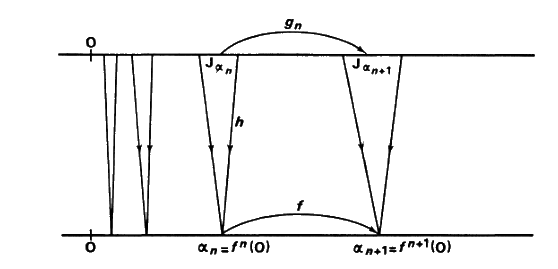
\includegraphics[scale=0.452]{diagram.png}
\captionof{figure}{\cite{herman} Schéma de la construction où $f=R_\alpha$}
\end{centering}

\subsection{Contre-exemple dérivable}

On considère toujours un homéomorphisme croissant $g_n$ de $I_n$ sur $I_{n+1}$, prolongé en $g_{n,p} = g_n +p$ sur $I_{n,p}$. On va de plus imposer que $g_n$ soit un difféomorphisme de classe $\mathcal{C}^1$, vérifiant : \\

$(*) \begin{cases}\ g_n'(x)=1 \ \text{ si } x \in \partial I_n \\ \displaystyle \lim_{n \to \pm \infty}\sup_{x\in I_n}|g_n'(x)-1|=0 \end{cases}$ \\

On considèrera enfin les fonctions $g_n'$ prolongées continuement sur tout l'intervalle [0,1], en les prenant constantes égales à 1 sur le complémentaire de $I_n$

\begin{lemma}$\displaystyle g_n : x \mapsto b_{n+1} + \int_{b_n}^x 1 + \frac{6}{l_n^2}(\frac{l_{n+1}}{l_n} -1)(t-b_n)(c_n-t)\mathrm{d}t$ vérifie la condition $(*)$.
\end{lemma}

\textbf{Preuve :} $g_n$ est un $\mathcal{C}^1$ difféomorphisme car sa dérivée est strictement positive. De plus, on a :
\begin{eqnarray*}
\int_{b_n}^{c_n} 1 + \frac{6}{l_n^2}(\frac{l_{n+1}}{l_n} -1)(t-b_n)(c_n-t)\mathrm{d}t &=& l_n +  \frac{6}{l_n^2}(\frac{l_{n+1}}{l_n} -1)\int_{b_n}^{c_n} (t-b_n)(c_n-t)\mathrm{d}t \\
&=& l_n +  \frac{6}{l_n^2}(\frac{l_{n+1}}{l_n} -1) \left [\frac{u^2}{2}l_n - \frac{u^3}{3}\right ]^{l_n}_0 \\
&=& l_n +  \frac{6}{l_n^2}(\frac{l_{n+1}}{l_n} -1) \frac{l_n^3}{6} = l_{n+1}
\end{eqnarray*}

Donc $g_n$ envoie bien $I_n$ sur $I_{n+1}$. La première condition de $(*)$ est immédiate, la seconde découle du fait que pour $x\in I_n$ : $ \displaystyle |g_n'(x) -1| \leq 6(\frac{l_{n+1}}{l_n} -1) \to 0 $ quand $n\to \pm \infty$ par hypothèse. \\ \qed
\begin{lemma}
La fonction $\eta$ qui coïncide avec $g_n'$ sur $I_n$ et qui vaut $1$ ailleurs est continue et vérifie $\displaystyle \eta =  1 + \sum_{n \in \mathbb{Z}} (g_n'-1)$
\end{lemma}

\textbf{Preuve :} 

%On va montrer le résultat en utilisant la caractérisation séquentielle. Soit $x \in [0,1]$, et $(x_j)_{j\in \mathbb{N}}$ qui tend vers $x$.
%
%\underline{1er cas} : si il existe $n$ tel que $x \in \overset{\circ}I_{n}$, alors à partir d'un certain rang la suite  $(x_j)_{j\in \mathbb{N}}$ est dans $I_n$, et la continuité de $\eta$ se déduit de celle de $g_n'$. \\
%
%\underline{2ème cas} : si il existe $n$ tel que $x \in \partial I_{n}$, on va montrer que, sous réserve d'existence, la suite extraite $(x_{\varphi(j)})_{j\in \mathbb{N}}$ des termes dans $\displaystyle \bigcup_{n \in \mathbb{Z}} I_{n}$, et celle $(x_{\phi(j)})_{j\in \mathbb{N}}$ des termes qui n'y sont pas, ont une même limite par $\eta$ qui vaut $1=\eta(x)$. Par définition, on a $\forall j \in \mathbb{N}, \eta(x_{\phi(j)}) = 1$, ce qui donne une première limite.

En différenciant les cas $x \in I_n$, et $\displaystyle x\in [0,1] \setminus \bigcup_{n \in \mathbb{Z}} I_n$, l'égalité ponctuelle est immédiate. On va de plus montrer que la convergence est uniforme, ce qui donnera la continuité de $\eta$. \\ 
Soit $N \in \mathbb{N}$, et $x\in [0,1]$, on a : $\displaystyle \sum_{|k| \geq N} (g_n'(x)-1)= \begin{cases} g_n'(x)-1 \ \text{ si il existe } n \text{ tel que } x\in I_n \text{ et } |n|\geq N\\ 0 \end{cases}$ \\
Dans tous les cas, $\displaystyle \sup_{x\in [0,1]} \left | \sum_{|k| \geq N} (g_n'(x)-1) \right | \leq \sup_{|n| \geq N} |g_n'(x) -1|$. Or par hypothèse sur les dérivées, ce majorant tend vers $0$ et donc la convergence est uniforme. \\ \qed \\

La fonction $g$ admet comme dans la partie précédente un prolongement en homéomorphisme de [0,1] mais on a cette fois le résultat plus fort suivant :

\begin{theorem}
$g$ est un difféomorphisme de classe $\mathcal{C}^1$ qui vérifie $\rho(g)=\alpha$ mais n'est pas conjugué à $R_\alpha$.
\end{theorem}


\textbf{Preuve :} Le seul point qui ne découle pas du \hyperref[th:cont]{Théorème 1.2} est que $g$ est un $\mathcal{C}^1$-difféomorphisme. Pour montrer cela, on commence par remarquer que $g$ est d'une part continue, et que d'autre part $g$ est un $\mathcal{C}^1$-difféomorphisme sur $\displaystyle U := \bigcup_{n,p\in \mathbb{Z}} I_{n,p}$ qui est de mesure pleine dans $\mathbb{R}$. \\
Alors, si $A$ est un borélien de mesure de Lebesgue nulle, on a $\lambda(g(A)) \leq \lambda(g(A\cap (\mathbb{R} \setminus U))) + \lambda(g(A\cap U))$. 
Or le premier terme est nul car $\mathbb{R} \setminus U$ est stable par $g$ et de mesure nulle, et le second terme est nul par théorème de changement de variable, $g$ étant un $\mathcal{C}^1$-difféomorphisme sur $ U $, et $A$ de mesure nulle. \\

On en déduit que la mesure de Stieltjes associée à $g$ est absolument continue par rapport à la mesure de Lebesgue. Ainsi $g$ admet une dérivée de Radon-Nikodym $\mu \in \mathcal{L}^1(\mathbb{R})$, telle que $g(x) = g(0) + \displaystyle \int_0^x \mu(t) \mathrm{d}t$. Mais alors $\mu$ est presque partout égale à $g_n'$ sur les $(I_{n,p})_{p\in \mathbb{Z}}$ d'après la théorie des points de Lebesgue, i.e presque partout égale à $\eta$ car $U$ est de mesure pleine, et on a finalement : $g(x) = g(0) + \displaystyle \int_0^x \eta(t) \mathrm{d}t$. \\
On en déduit que $g$ est un homéomorphisme $\mathcal{C}^1$ de $\mathbb{R}$ à dérivée non nulle, et donc un $\mathcal{C}^1$-difféomorphisme. \\ \qed

\subsection{Régularité hölderienne}

Soit $w:[0, 1] \mapsto [0, 1]$ un module de continuité, on considère l'ensemble des fonctions continue pour ce module, $\displaystyle\mathcal{C}^w(\mathbb{T}) := \left\{ \varphi \in \mathcal{C}^0(\mathbb{T}) \ \left| \ \sup_{ 0<|x-y|\leq 1}  \frac{|\varphi(x)-\varphi(y)|}{w(|x-y|)} < +\infty \right. \right\} $ \\

En considérant la fonction $g$ construite dans la partie précédente, on a le lemme :

\begin{lemma}
$ \displaystyle \sup_{n\in \mathbb{Z}} \left |\frac{l_{n+1}}{l_n}-1 \right |\frac{1}{w(l_n)} <+ \infty \Rightarrow g' \in \mathcal{C}^w(\mathbb{T})$
\end{lemma}

\textbf{Preuve :} On suppose sans perte de généralité que $w(x)/x$ est décroissante. En reprenant le $g_n'$ de la construction précédente, on constate que :  \\

$\displaystyle |g_n''(t)| = \frac{6}{l_n^2}(\frac{l_{n+1}}{l_n}-1)|(c_n-t + b_n -t)| \leq  \frac{3}{l_n}(\frac{l_{n+1}}{l_n}-1) $ \\

L'inégalité des accroissements finis donne donc : \\

$\displaystyle \sup_{0<x-y\leq 1} \left | \frac{g_n'(x) - g_n'(y)}{w(x-y)}\right | \leq \left | \frac{l_{n+1}}{l_n}-1\right | \frac{3}{w(l_n)} < +\infty$, et on en déduit que $g' \in \mathcal{C}^w(\mathbb{T})$ car $g'-1$ est limite uniforme de $\displaystyle  \sum_{k = -n}^n (g_k'-1)$, et les fonctions dans la somme ayant des supports disjoints 2 à 2, on a :\\

$\displaystyle  \left | \sum_{k = -n}^n (g_k'-1) \right |_{\mathcal{C}^w} \leq \sup_{n \in \mathbb{Z}} |g_n' -1|_{\mathcal{C}^w} \leq \frac{3}{l_n}(\frac{l_{n+1}}{l_n}-1) < + \infty $

~ \\

\underline{Rq }: Ce résultat est en fait une équivalence. \\

La suite $ \displaystyle l_n := \frac{c}{(|n|+k)(log(|n| + k)^{1+\epsilon}}$ vérifie le critère du lemme 1.5 pour le module $w(x)=O(x^{1-\epsilon'})$, pour tout $\epsilon' > \epsilon$


\newpage
\printbibliography[heading=bibintoc, title={Références}]

\end{document}
